% WHAT?
% WHY?
% User story compatibility 

Generally, the design of the user interface for the web application is an integration of the principles previously described with core design elements of web and the twitter bootstrap element library. 

\subsection{Layout and Structure}
The structure of the application is in most cases shallow, the navigational depth is usually two steps but sub views with modal views may result in a depth of 3. There are three types of views which are hierarchical in some way, main views contain sub views and modal views, sub views may contain modal views.

\begin{itemize}
    \item \textbf{Navigation bar:}
A navigation bar is a menu that contains an overview of the functionality in the form of, in this case, tabs that leads the user to other views and that is always visible for the user to allow easy navigation. The navigation bar for the application can be seen in \autoref{adm_web_annotationView1}. Since the most important parts of the application is to be able to upload, process and convert files, these are each a natural part of the navigation bar (although conversion is not yet implemented and therefore not shown in the figure).

\begin{figure}
 \centering
 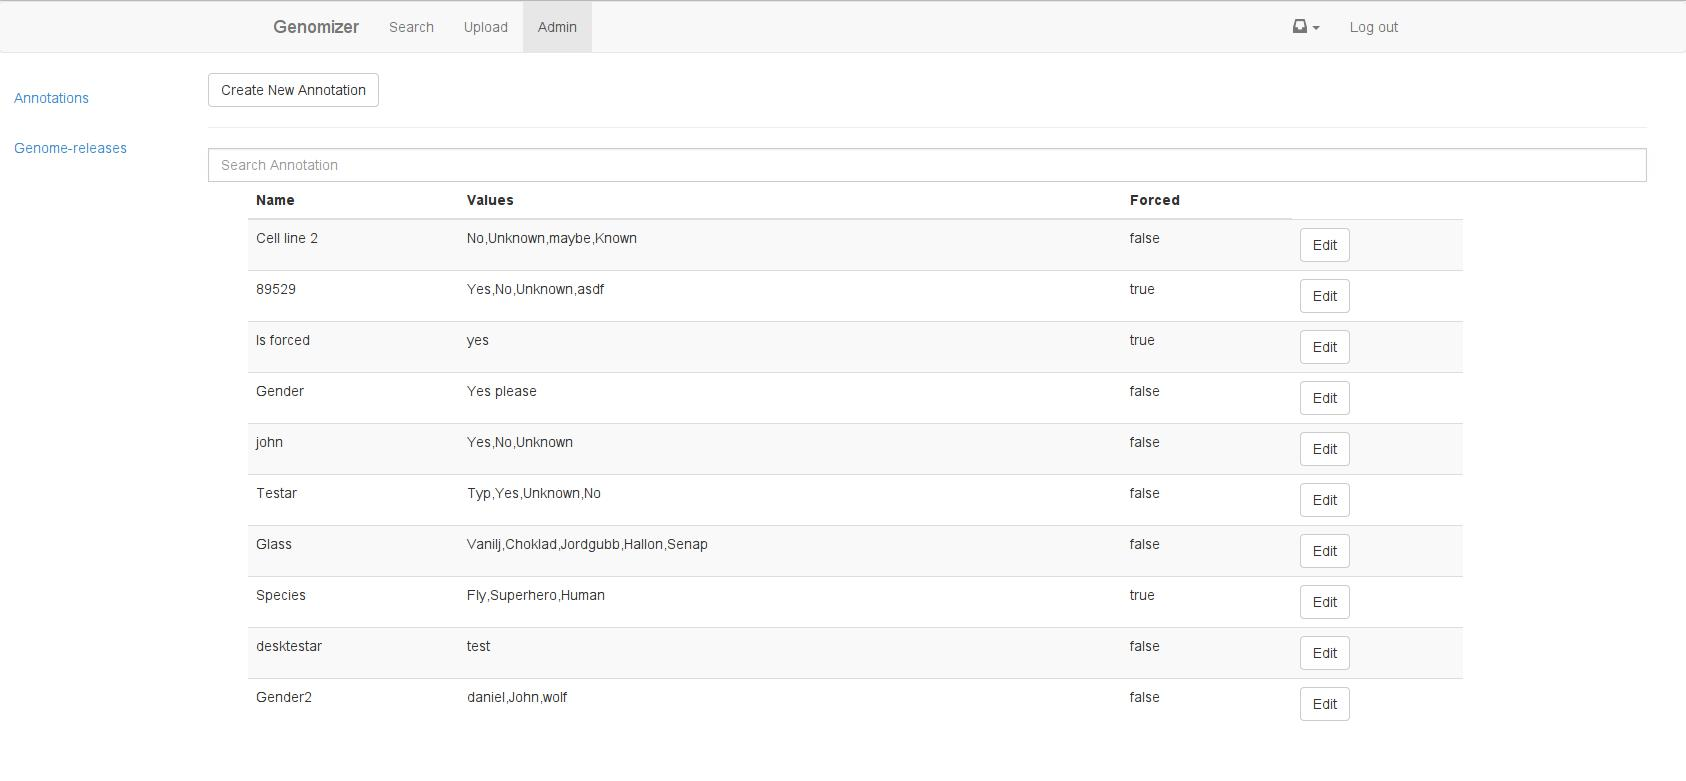
\includegraphics[trim=40 260 45 50, clip, width=0.8\textwidth]{web_SysadminAnnotationView.jpg}
 \caption{\footnotesize  The web client navigation bar.}
 \label{adm_web_annotationView1}
\end{figure}

	\item \textbf{Main views:}
A main view covers the entire page except for the navigation bar. The structure among main views is shallow and the user may freely navigate between all main views using the navigation bar. Typically a main view contains a toolbar and a set of panels. \autoref{adm_web_annotationView2} shows the administration main view.

\begin{figure}
 \centering
 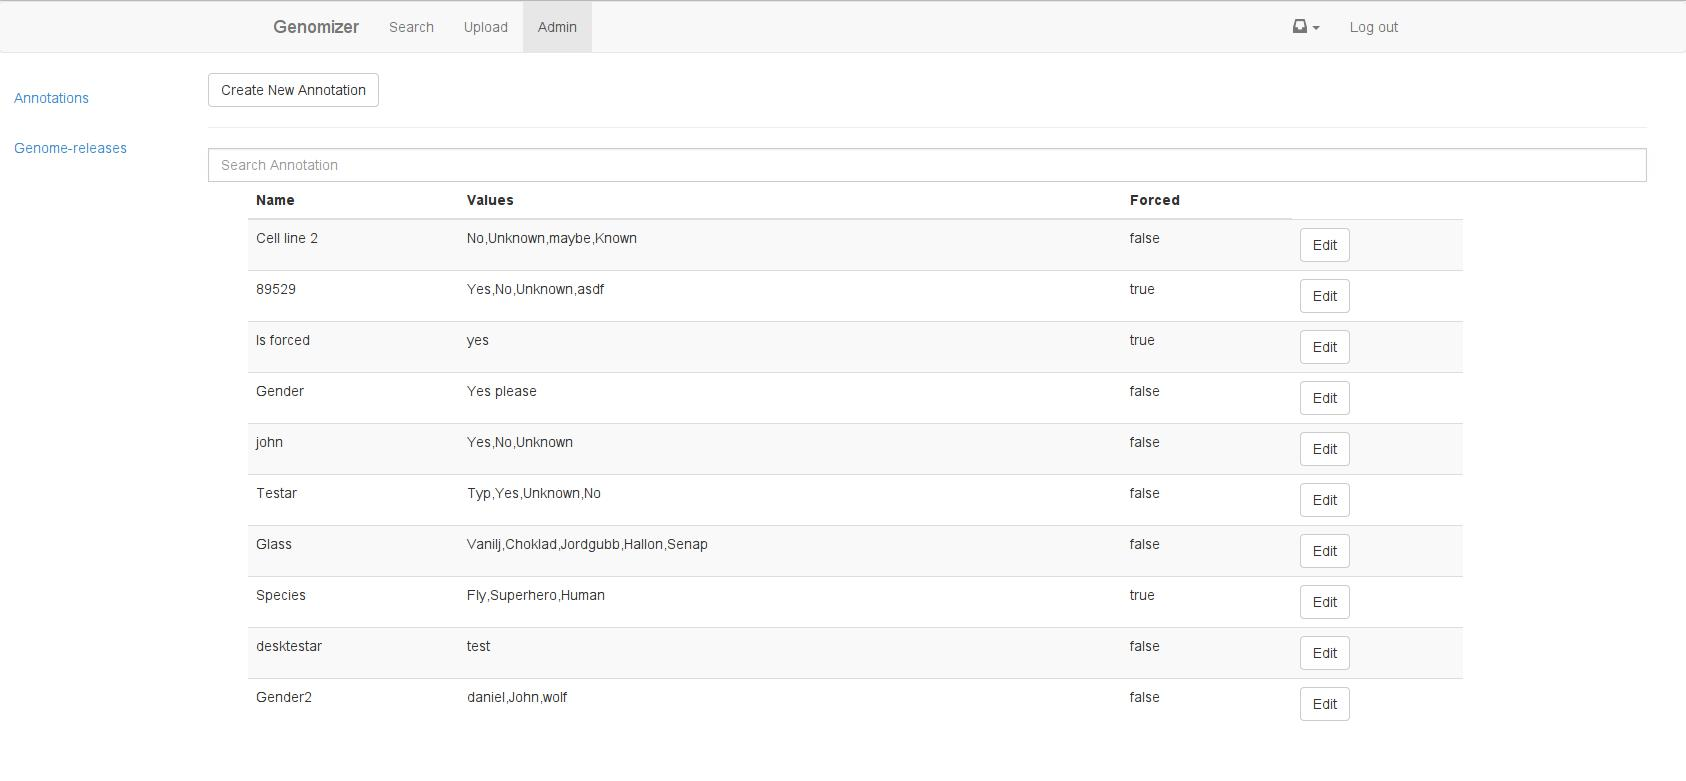
\includegraphics[width=\textwidth]{web_SysadminAnnotationView.jpg}
 \caption{\footnotesize The web client administrator main view.}
 \label{adm_web_annotationView2}
\end{figure}

	\item \textbf{Sub views:}
A sub view is a part of a main view. In the case of the administrator view seen in \autoref{adm_web_annotationView2}, the main view has a vertical navigation bar on the left side used to navigate between sub views, sub views may not be directly navigated outside of its main view. The user may navigate to other main views from a sub view. Except for the sub navigation bar the sub view covers the entire main view, replacing its content, as does the annotation view in this case.

	\item \textbf{Modal views:}
Modal views are opened on top of the current main view and are used for specialized operations. Modal views can be navigated to using buttons inside main views and sub views. Usually the user will be taken back to the previous view when the modal is closed but navigation in a sequence of modal views could be implemented in the future. An example
of a modal view is the login view seen in \autoref{fig:web_search_login1}.

\begin{figure}
\centering
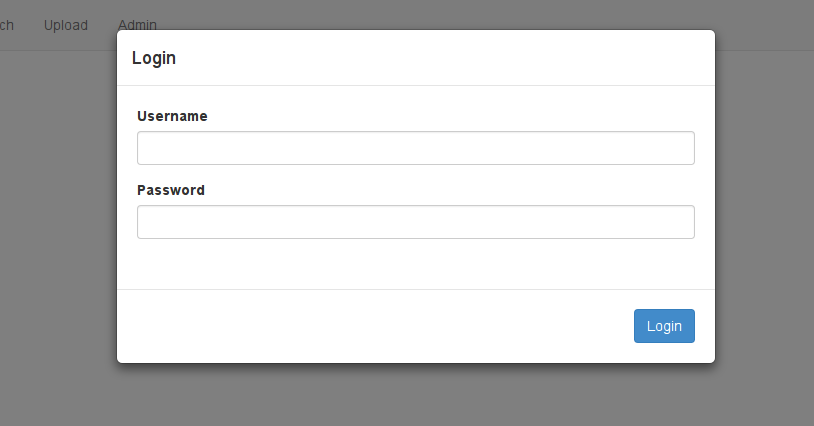
\includegraphics[width=0.8\textwidth]{web/manual/web_login.png}
\caption{\footnotesize The login modal.}
\label{fig:web_search_login1}
\end{figure}

    \item \textbf{Panels:}
Content that belongs together is grouped using so bootstrap panels. Main views and sub views should contain one or more panels.
    
    \item \textbf{Toolbars:}
In main views and sub views we use a toolbars where operation controls available to the user are presented, for example, add and search experiment functionality in the upload view.
    
    \item \textbf{Popovers:}
Elements that belong to a view but have no need to be visible at all times are shown in bootstrap popovers. Popovers that do not belong to a specific view may be placed in the navigation bar, that is, the main menu.
\end{itemize}

\subsection{Colors}
Grayscale colors are mostly used, black or dark gray is used for text, icons and borders while white or light gray is used for backgrounds. Colors of different hues are used to distinguish elements from each other and to highlight important elements. Colors with high saturation are reserved for smaller elements while colors with lower saturation can be used regardless of element size. Light gray of varying brightness may also be used to highlight or distinguish elements.

\subsection{Icons}
Buttons that perform actions should always contain an icon as well as text so that the experienced user may more quickly desired actions by identifying buttons at a glance instead of having to read the button text. 

\subsection{Batching}
For operations performed on objects that there are multiples of e.g. experiments or files, let the user perform these operations on multiple objects at the same time in cases where it makes sense using checkboxes.

\subsection{Processing}
The interaction flow of the processing is adapted from the actual processing 
steps in order to help the researchers by increasing usability through providing
a well-known but more optimized approach.

After having chosen an experiment for processing and entered the processing 
view, the user can choose the processing steps wanted and enter the correct
files and parameters for each processing step as shown in 
\autoref{fig:web_process_processOverview}.

\begin{figure}[h]
    \centering
    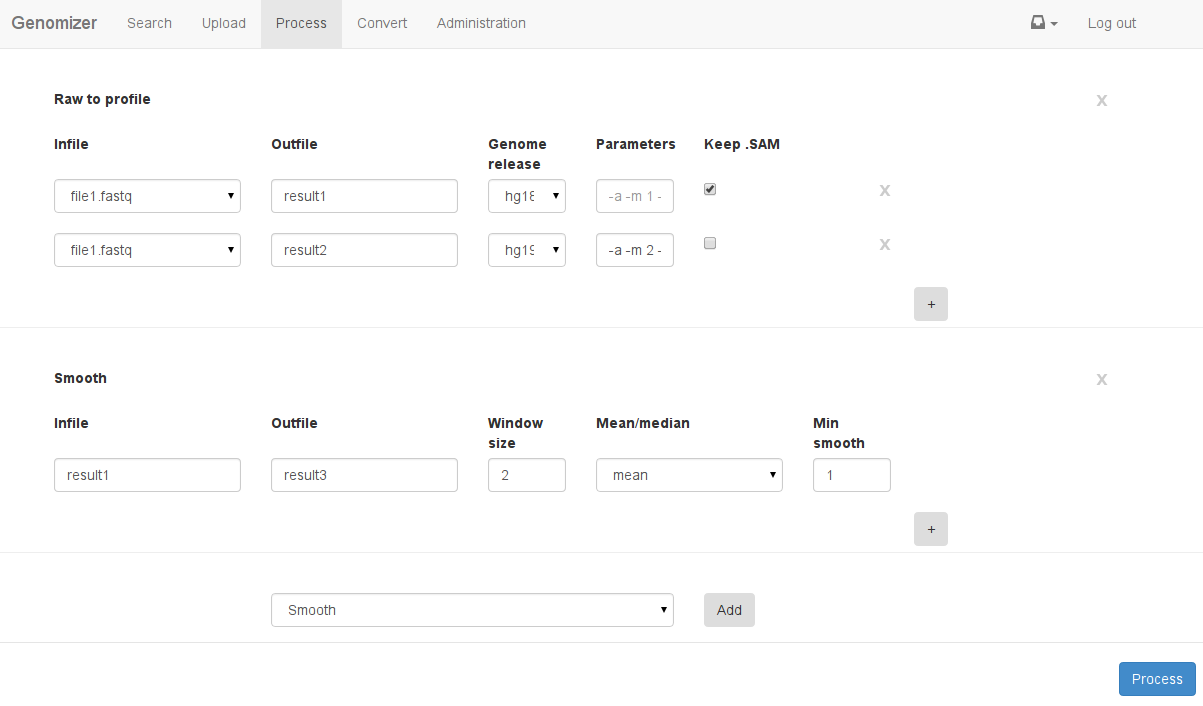
\includegraphics[trim=0 0 85 0, clip, width=1\textwidth]{web_process_processOverview.png}
    \caption{\footnotesize Files selected for upload.}
    \label{fig:web_process_processOverview}
\end{figure}

\subsection{System administration}
The admin page is built up by a number of components: the main view, the side bar, the create annotation view, the edit annotation view and the genome-release view. The first one is the main view which consists of a sidebar and an empty div-tag. The empty div-tag is then replaced with the annotation list view which has a Create new annotation button and a list of the available annotations on the database with an option to edit. 

When the user clicks on for example Create New Annotation, the div tag in the main view is replaced with the create annotation view. The same goes for the Edit buttons on each annotation. This way we only have to render that specific div-tags current information and the sidebar is unaffected. 

The design is made so that the user should be able to avoid mistakes. For example in the create annotation page the user is not able to create an annotation without filling in all the fields. Futher more the field for Items in drop-down list is disabled if the user don't choose Drop-down list as the annotation type. 

In the Edit annotation view the same principles apply, but also there is a Delete Annotation button on this page which will delete the entire annotation from the database.For that reason we decided to ask if the user is sure of this action and of course made the button red.

The back buttons on the different views work as one would expect and the sidebar option Annotations takes the user back to the main adminview.

The sidebar item ''Genome-releases'' takes the administrator to the page for adding and editing genome-releases. This page have the same look and feel as the previous. The delete buttons are red and will prompt a confirmation-popup. 

The ''Select files to upload'' will as expected open the file explorer and the user chooses files according to normal operativesystem standards, then the ''Upload'' button will prompt the user for information about the files such as species and genomeversion before uploading. 